\documentclass[10pt]{article}

\usepackage{answers}
\usepackage{setspace}
\usepackage{graphicx}
\usepackage{enumitem}
\usepackage{multicol}
\usepackage{circuitikz}
\usepackage{adjustbox}
\usepackage{mathrsfs}
\usepackage{mathtools}
\usepackage{fancyhdr}
\usepackage{svg}
\usepackage[margin=1in]{geometry}
\usepackage{amsmath,amsthm,amssymb}
\usepackage[compact]{titlesec}
\titlespacing{\section}{0pt}{*0}{-10pt}
\titlespacing{\subsection}{0pt}{*0}{-10pt}
\titlespacing{\subsubsection}{0pt}{0pt}{-10pt}
\parindent 0in
\parskip 12pt
\setlength{\headsep}{-10pt}
\setlength{\topskip}{0pt}
\setlength{\topmargin}{0pt}
\setlength{\topsep}{0pt}
\setlength{\partopsep}{0pt}
\geometry{margin=1in, headsep=0.25in}
\setlist[itemize]{label={--}, topsep=-10pt, noitemsep}
\setlist[enumerate]{topsep=-10pt, noitemsep}
\newcommand{\N}{\mathbb{N}}
\newcommand{\Z}{\mathbb{Z}}
\newcommand{\C}{\mathbb{C}}
\newcommand{\R}{\mathbb{R}}


\pagestyle{fancy}
\lhead{Aditya Arora}
\rhead{page \thepage}
\cfoot{ECE 222 Digital Computers}
\renewcommand{\headrulewidth}{0.2pt}
\begin{document}
\section*{Basic Processing Unit}
Three main parts of the CPU:
\begin{enumerate}
    \item Control Unit
    \item ALU
    \item Register file
    \item Processor memory interface
    \item instruction address generator (with PC and IR)
\end{enumerate}
\subsection{Datapath}
The \underline{datapath}: It is a collection of Functional units, registers, memory interfaces that perform every instruction in the ISA\\
\begin{itemize}
    \item The pipeline is distributed into 5 stages along the datapath
    \begin{enumerate}
        \item Fetch: Get the instruction pointed to by the PC, store it in IR\\
        Memory address $\leftarrow$ [PC], Read memory, Wait for MFC, IR $\leftarrow$ Memory data, PC $\leftarrow$[PC] + 4
        \item Decode: The instruction is decoded and the source registers are read\\
        RA $\leftarrow$ [Address A],
        RB $\leftarrow$ [Address B],
        Op Code $\leftarrow$ [depending on instruction]\\
        Note all these addresses locations are dependent on the type of instruction as below
        \item Execute: The computation specific for the instruction is performed.
        RZ $\leftarrow$ computation result, RM $\leftarrow$ RB\\
        An immediate value is selected from MuxB if the need be. RM is made RB if the instruction is one involving memory read or write (in that case RZ hold the effective address)
        \item Memory:  If instruction is a memory instruction then perform it in this stage. \\
        If not memory: RY $\leftarrow$ RZ\\
        If Load: RY $\leftarrow$ memory data\\
        If Store: RY $\leftarrow$ RZ (for writeback just in case)\\
        If Branch: RY $\leftarrow$ Return address [to be written to link register]
        \item Write-Back: The result of the instruction’s operation is stored in the destination register. Address of C determined by corresponding IR bits\\
        addressC $\leftarrow$ RY
    \end{enumerate}
    \item There are multiple inter-stage buffers that pass information along
    \item There are also multiple control signals responsible for controlling the flow of information.
    \begin{enumerate}
        \item generate individual signals per step of instruction in the data-path
        \item control memory access (read/write)
        \item determine which registers to be accessed/written to
        \item determine MUX control signals
        \item determine branch flow by controlling PC signals
        \item determine operation for the ALU
        \item determine the type of the instruction:
        \begin{enumerate}
            \item Register Operand format $$R_{src1}(31-27)|R_{src2}(26-22)|R_{dst}(21-17)|OP\; code(16-0)$$
            \item Immediate Operand format $$R_{src1}(31-27)|R_{dst}(26-22)|Immediate\; operand(21-6)|OP code(5-0)$$
            \item Call format $$Immediate\; operand(31-6)|OP code(5-0)$$
        \end{enumerate}
    \end{enumerate}
\end{itemize}
\newpage
\subsection{Control Signals}
The \underline{control circuitry}: implements the decode stage of the instruction execution, and sets the appropriate signals at each stage to regulate the flow of data.
\begin{itemize}
    \item Register File
    \begin{enumerate}
        \item RF\_write: When writing to register file it is set to 1
        \item C\_select: Depending on instruction format
        \begin{itemize}
            \item R-type: dest is $IR_{21-17}$
            \item I-type: dest is $IR_{26-22}$ \item Branch: dest is \texttt{LINK}
        \end{itemize}
    \end{enumerate}
    \item ALU
    \begin{enumerate}
        \item B\_select: 0 for RB, 1 for immediate
        \item ALU\_op: k-bit control signals (for each type of operation)
        \item Condition signals: Output of ALU, set by the ALU, and monitored for branch conditions
    \end{enumerate}
    \item Memory and IR:
    \begin{enumerate}
        \item MEM\_read: Set when reading
        \item MEM\_write: Set when writing
        \item IR\_enable: loads intruction into IR, and activated in Fetch stage after MFC is asserted
        \item MA\_select: choose between RZ and PC for choosing the address input to memory
        \item MFC: stall signal, if cache hit then asserted in same clock cyle as request, otherwise instruction stalled until memory access complete
    \end{enumerate}
    \item Instruction Address Generator:
    \begin{enumerate}
        \item INC\_select: Chooses between +4 and branch offset for PC incrementation
        \item PC\_select: Chooses between subroutine RA(0) and incremented PC(1), and needs PC\_enable to be on
    \end{enumerate}
\end{itemize}
There are 2 ways to generate these control signals:
\begin{enumerate}
    \item
    \begin{minipage}{0.60\textwidth}
         \underline{Hardwired control:} Decoder interprets Op-code and address mode in IR, while step counter (modulo 5) sets  T\# to indicate which stage to execute, while control signal generator is a combinational circuit responsible for generating the right signals
        \end{minipage} \hfill
        \begin{minipage}{0.35\textwidth}
        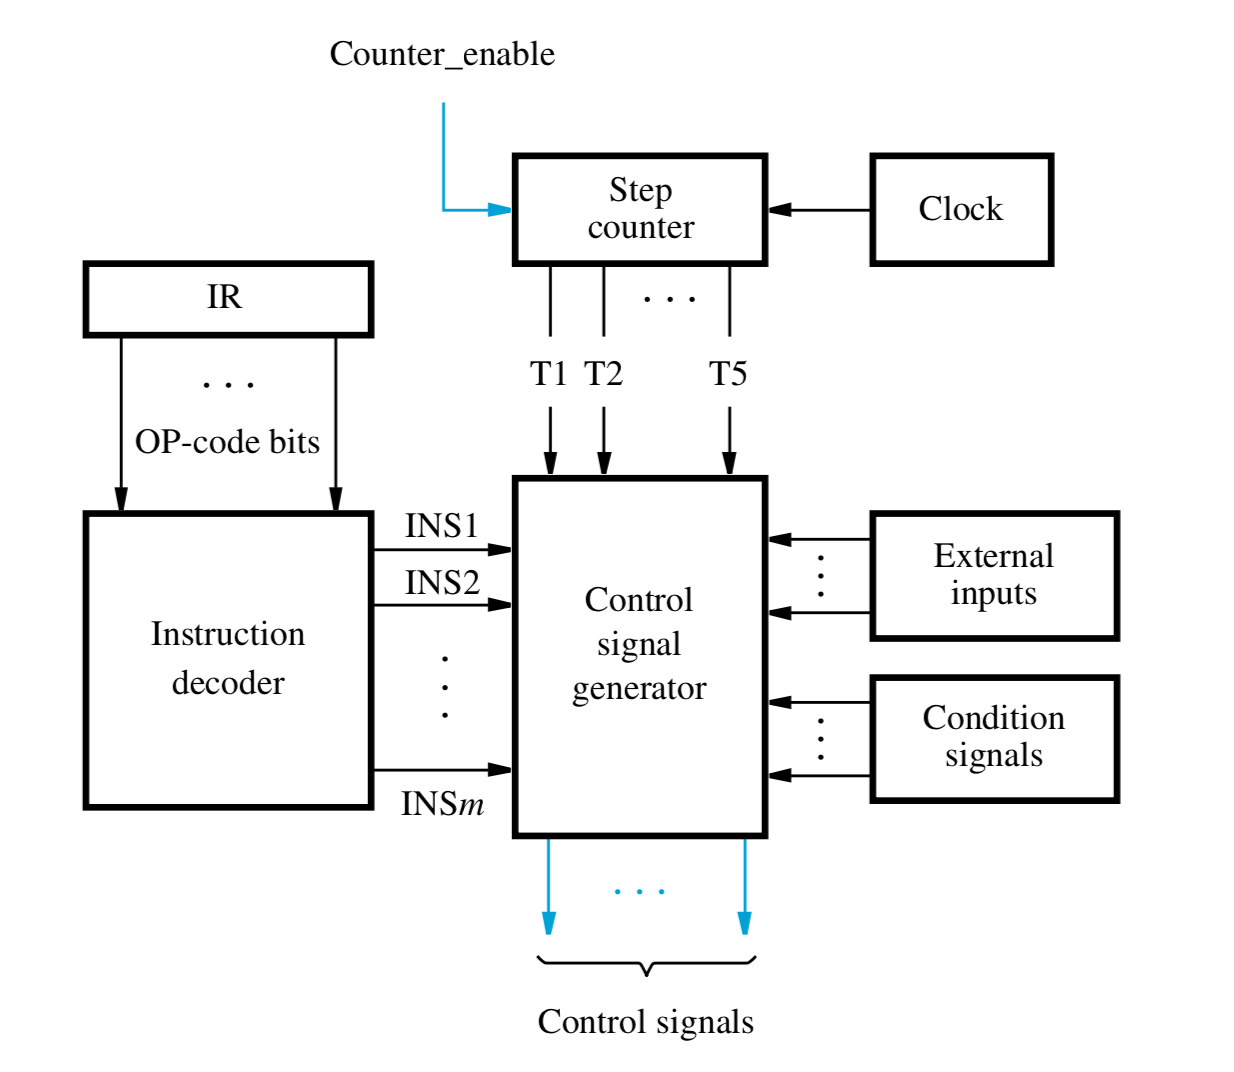
\includegraphics[width=0.8\textwidth]{bpu/hardwired.png}
        \end{minipage}
    \item \underline{Microprogrammed control:} Using software (not in TB or notes)
\end{enumerate}
\end{document}
